The Single Instruction Multiple Data (SIMD) architecture was popular in the
1990s.
%
With SIMD architecture, all processing units execute identical instructions
cycle by cycle, but they access different local data from their private 
local memory.
%
All processing units are also connected in a net structure, allowing
communication between them.
%
Figure~\ref{fig:simd1} illustrates an example SIMD architecture.

\begin{figure}[p]
    \centering
    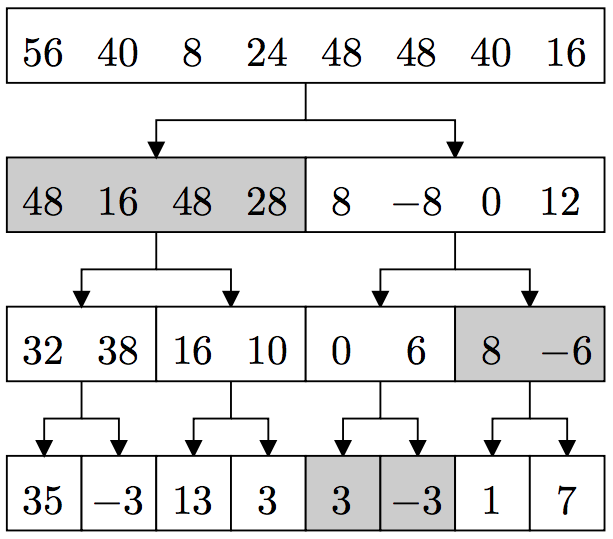
\includegraphics[width=0.8\textwidth]{fig/example1.png}
    \caption{An example of DWT on a signal with 8 elements.}
    \label{fig:simd1}
\end{figure}


\cite{lee1994parallel}

